\documentclass[a4paper,twoside,kul]{kulakreport} %options: kul or kulak (default)

\usepackage[english]{babel}
\usepackage[nosort]{cite}
\usepackage{textcomp}
\usepackage{graphicx}
\usepackage{subcaption}
\usepackage{fullpage}
\usepackage{cleveref}
\usepackage{etoolbox}

\makeatletter
\patchcmd{\chapter}{\if@openright\cleardoublepage\else\clearpage\fi}{}{}{}
\makeatother

\faculty{Master of Mobility and supply chain engineering}
\group{Public Transportation, Design and Management [H0T93a]}
\title{Analysis: Commuting to Berlin}
\subtitle{Exam assignment}
\author{Edward Vanlerberghe and Seppe Vilain}
\institute{KU Leuven}
\date{Academiejaar 2021-2022}
\address{
   KU Leuven         \\
   Faculty of Engineering Science \\
   Kasteelpark Arenberg 1 bus 2200\\
   B-3001 LEUVEN             \\
   \texttt{edward.vanlerberghe@student.kuleuven.be} \\
   \texttt{ seppe.vilain@student.kuleuven.be}
   }

\begin{document} % hier begint de eigenlijke inhoud van het document

\titlepage
\tableofcontents

\clearpage
\chapter*{Introduction}
Inleidende tekst.

\clearpage
\chapter{Types of transport}
\begin{figure}[h]
	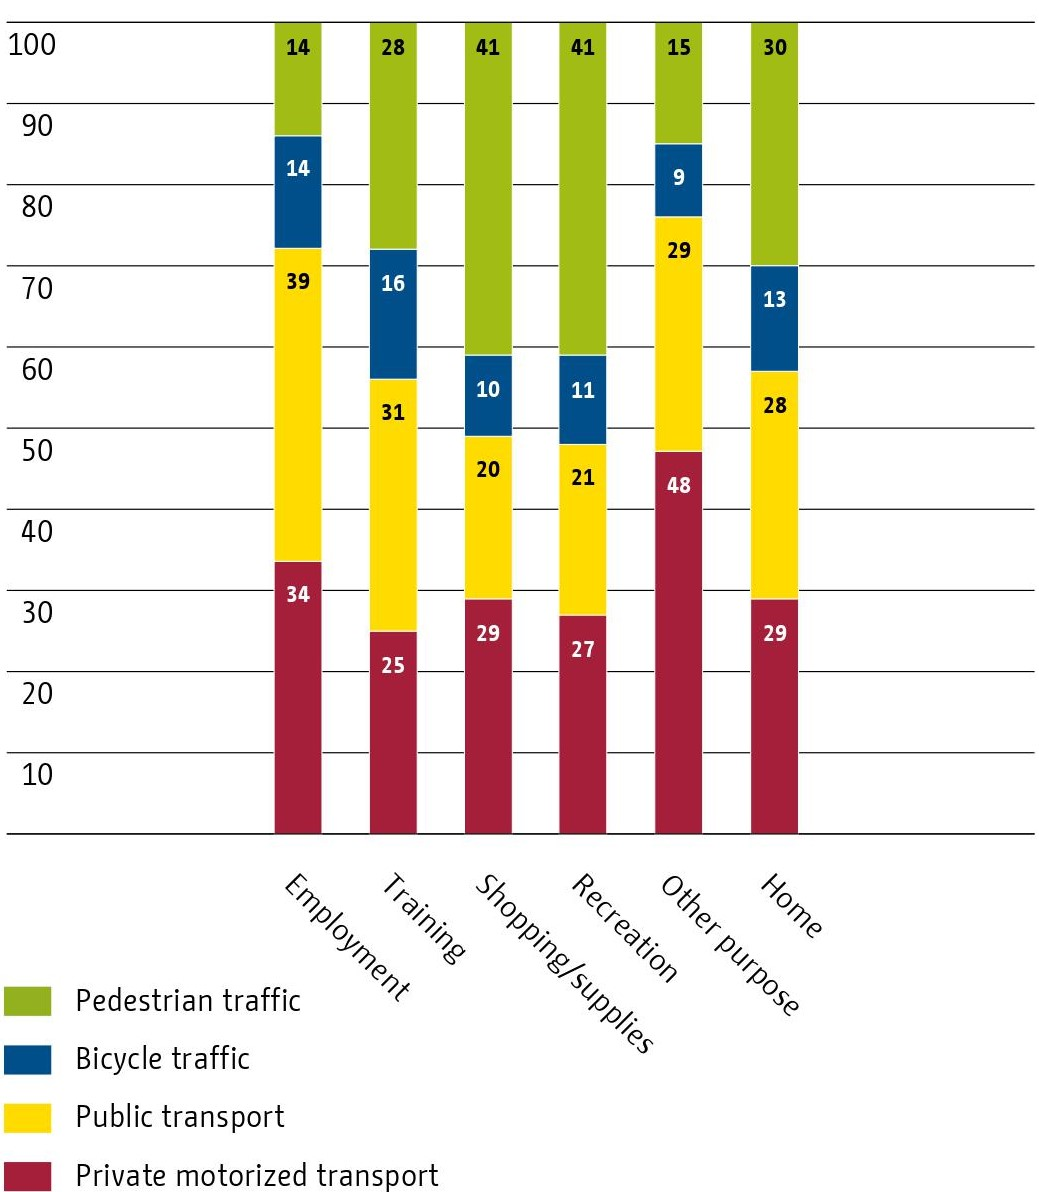
\includegraphics[width=0.5\textwidth]{MobilityInTheCityJPG/Graphs/UseOfTransportPurpose.jpg}
	\centering
	\caption{Use of transport mode by purpose of journey.\cite{MobilityCity}}
\end{figure}
\section{Car}

With a length of approximately 5400 km of roads the car remains the most used mean of transport to commute to work. Improving the roads and making more parking spaces available makes the car an attractive option. However, only 20\% of the road vehicles travelling in Berlin are private cars. The other 80\% cars are vehicles belonging to flexible, non-binding schemes and with a fixed pick-up point.  The main traffic roads\footnote{Main traffic roads: they have a total length of 160 km.} ensures that people coming from Berlin's suburbs or nearby cities reach the minor roads efficiently (Figure \ref{motorways}). The vast majority of these minor roads (370 km) have a speed limit of 30 km/h upon them, which is due to safety reasons and noise control\cite{MobilityCity}. 

The demand for parking spaces is significantly higher than the supply, but this is where Berlin's parking policy plays a big role. A 100,000 parking spaces across 45 parking zones provides a reasonable amount of place to store the commuters vehicle during day or night. Nevertheless parking in Berlin can get expensive. If you live in Berlin and you want to park in your neighbourhood you need a permit\footnote{In German: Bewohnerparkausweis} which costs \texteuro20.40 and is valid for two years. Otherwise you have to pay at the parking meter. Outside the \textit{Ringbahn}\footnote{Berliner Ringbahn: a 37.5 km long circle route around Berlin's inner area, on the Berlin S-Bahn network.} you can park for free. Other costs like car insurance (\texteuro100 to \texteuro1000 per year), vehicle tax\footnote{Kraftfahrzeugsteuer} (around \texteuro100 per year), fuel, a vehicle inspections per two years (\texteuro100), maintenance and repairs make the use of the car for commuting an expensive option\cite{CostCars}.

\begin{figure}[h]
	\begin{minipage}[c]{0.4\linewidth}
		\centering
		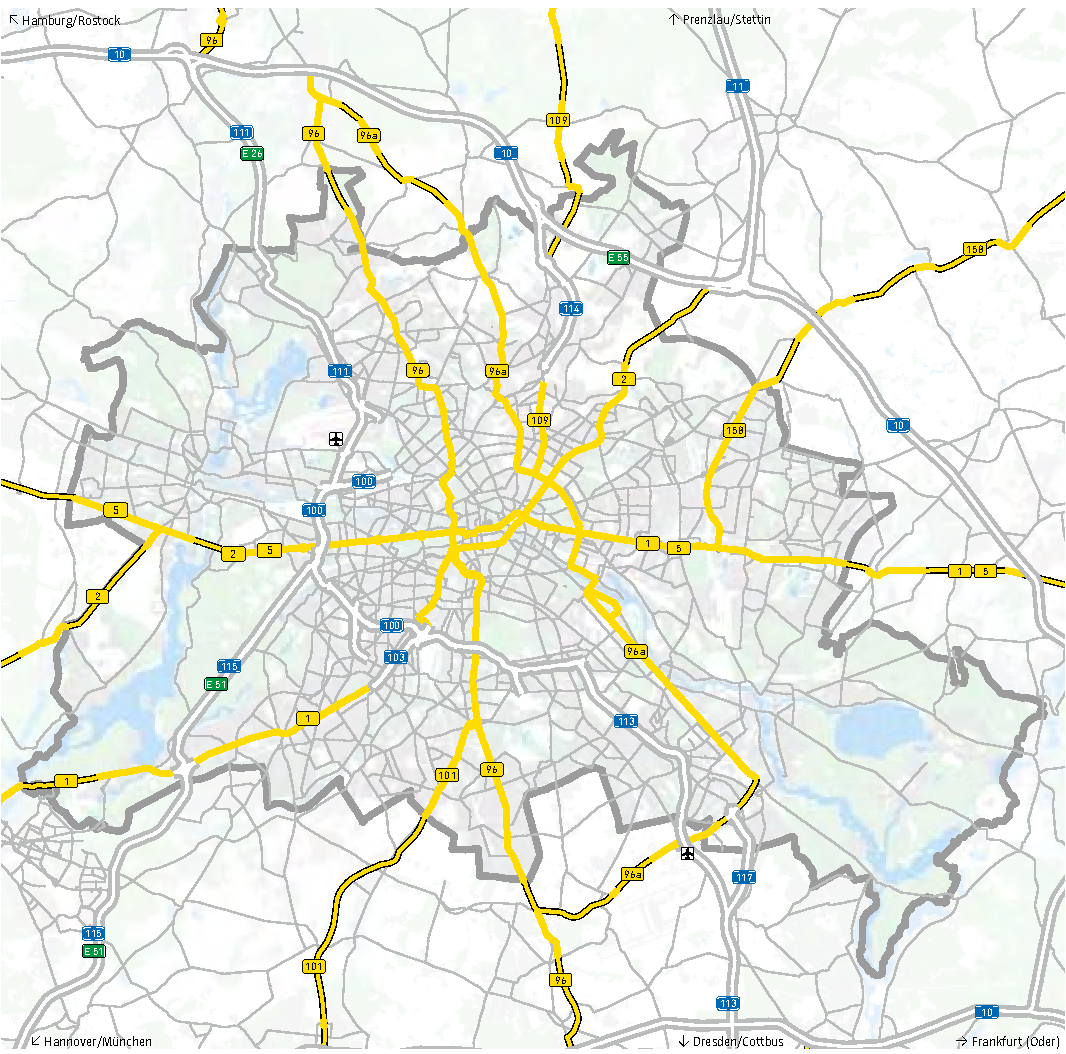
\includegraphics[height=7cm]{MobilityInTheCityJPG/Graphs/Motorways.pdf}
		\caption{Motorway and major road network}
		\label{motorways}
	\end{minipage}\hfill
	\begin{minipage}[c]{0.5\linewidth}
		\centering
		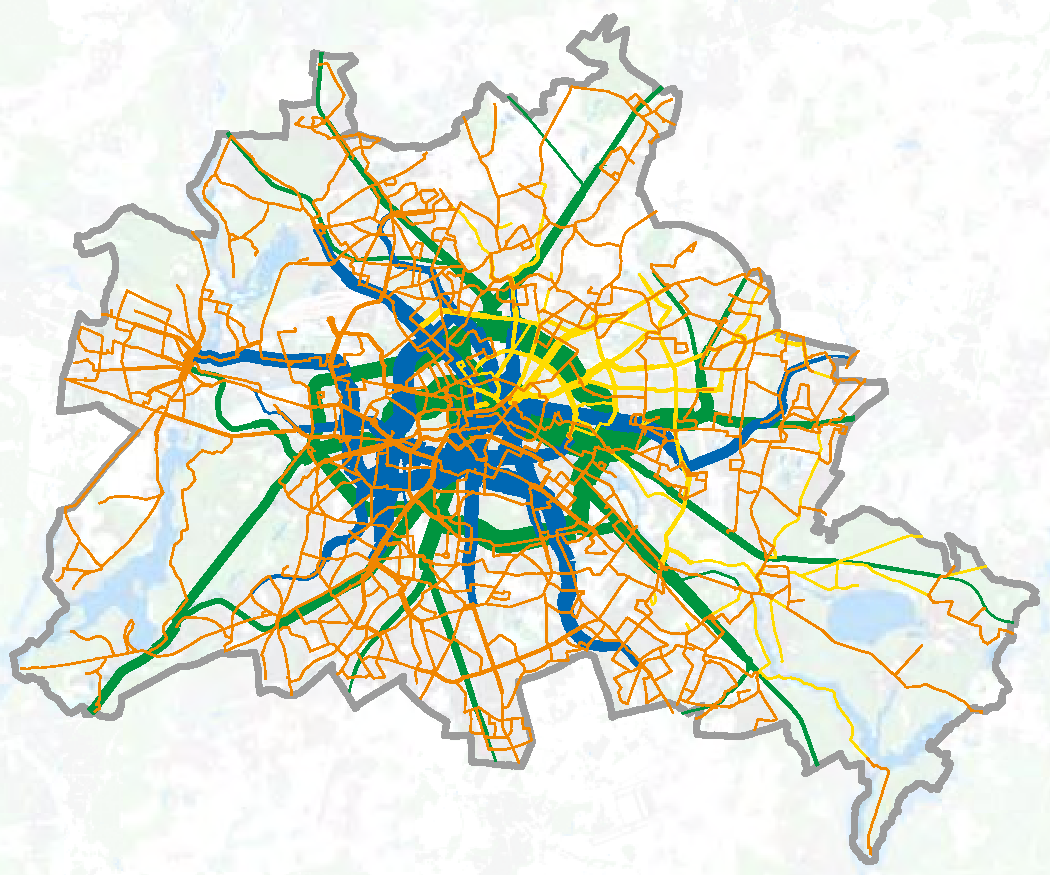
\includegraphics[height=7cm]{MobilityInTheCityJPG/Graphs/PTnetwork.pdf}
		\caption{Public transport network by transport mode}
		\label{ptnetwork}
	\end{minipage}
\end{figure}


\section{Bus}

The bus network consists of a large network that covers almost the entire city of Berlin (orange lines in Figure \ref{ptnetwork}). The network consists of 149 daytime and 63 night bus routes, seventeen MetroBus and 13 express routes.  The day lines connect the suburbs with the central city or S-Bahn and U-Bahn stations. The night bus lines replace partially certain U-Bahn lines and the most important day lines. The MetroBuses give service in areas that are poorly served by the U-Bahn and S-Bahn. They are designated as part of the \textit{MetroNetz} and serve 24 hours per day, seven days per week, in intervals of ten minutes. The X-buses (express) are faster routes which is accomplished through a small number of the more important stops on the route. By the greater distance between the stops, the buses lose less time on stopping the vehicle\cite{xpress}. \\

\subsection*{BVG}
The \textit{Berliner Verkhersbetriebe} (BVG\footnote{BVG: An abbreviation from the original company \textit{\textbf{B}erliner \textbf{V}erkehrs-Aktien\textbf{g}esellschaft}}) is the main public transport company of Berlin. It coordinates and develops the U-Bahn, tram, bus, replacement services and ferry networks\cite{BVG1}. With their 3,000 vehicles, they transported 1,064 million passengers in 2016 or more than 2.7 million passengers per day\cite{MobilityCity}.


\section{Tram}
 The tram network in Berlin was founded in 1865 and is hereby one of the oldest there is. After Melbourne and St. Petersburg, it's the largest tram system in the world. Since 1929, the BVG has operated the system\cite{tram}. By 1967, due to the Cold War and the division of Berlin in East and West Berlin, most tram lines that ran along West Berlin had closed, resulting in only two operational tram lines. The trace of the division is still visible, seeing that most tram lines are still in East Berlin\cite{tramz}. It's made of 22 lines and measuring almost 190 km in route length. Also here there are nine Metrotrams that give service 24 hours per day with small intervals\cite{tram}. 
 
\section{Train}
\subsection{S-Bahn}

Since 1930, the \textit{Berliner S-Bahn} has been operational in and around Berlin. This rapid transit railway system\footnote{Rapid transit: type of high-capacity public transport generally found in urban areas.} works complementary with the U-Bahn and connects the city centre with the suburbs. Through the high frequency and travel possibilities throughout Berlin and beyond, the S-Bahn has the characteristics of the combination between a commuter rail service and a rapid transit system. This railway system has three characteristics that make this public transportation mode unique. Vehicles that use the term S-bahn, are provided of a third-rail electrical power transmission\footnote{Third rail: A method of providing electric power to a train, through a semi-continuous rigid conductor placed alongside the rails of the track\cite{thirdRail}.}, the Berlin S-Bahn loading gauge\footnote{A loading gauge defines the maximum height and width for railway vehicles and their loads to ensure that they can pass safely through tunnels and under bridges\cite{gauge}.} and a communications-based train control system specific to the S-Bahn, in opposite of the usual automated mechanical train control system. The S-Bahn network consists of 16 lines serving 166 stations and has a total route length of 332 km. Three core lines can be seen when look at the S-Bahn: a central, elevated east-west line, a central, mainly underground north-south line and a circular line. All lines begin to disperse upward of the \textit{S-Bahn Ring}\cite{SBahn}. Per year the S-Bahn transports 334 million passengers and one million commuters per work day\cite{SBahnFIGURES}.\\

Opposed to trams and buses, which are operated by the BVG, the S-Bahn is part of the \textit{S-Bahn Berlin GmbH}, a company that is completely owned by the \textit{Deutsche Bahn}, a private, joint-stock and German railway company, with the Federal Republic of Germany being its single shareholder\cite{DB}.

\subsection{U-Bahn}

Together with the tram network and the S-Bahn, the U-Bahn is definitely the main means of transport in the German capital. The \textit{Untergrundbahn} opened in 1902 and serves currently 175 metrostations across nine lines, which make a total length of 155 km. The metro vehicles run every five minutes during the day, every ten minutes during the evening and from two to five minutes during peak hours. The U-Bahn is operated by the BVG\cite{UBahn}.

\section{Ticketing system and price}
\begin{figure}[h]
	\begin{minipage}[c]{0.4\linewidth}
		\centering
		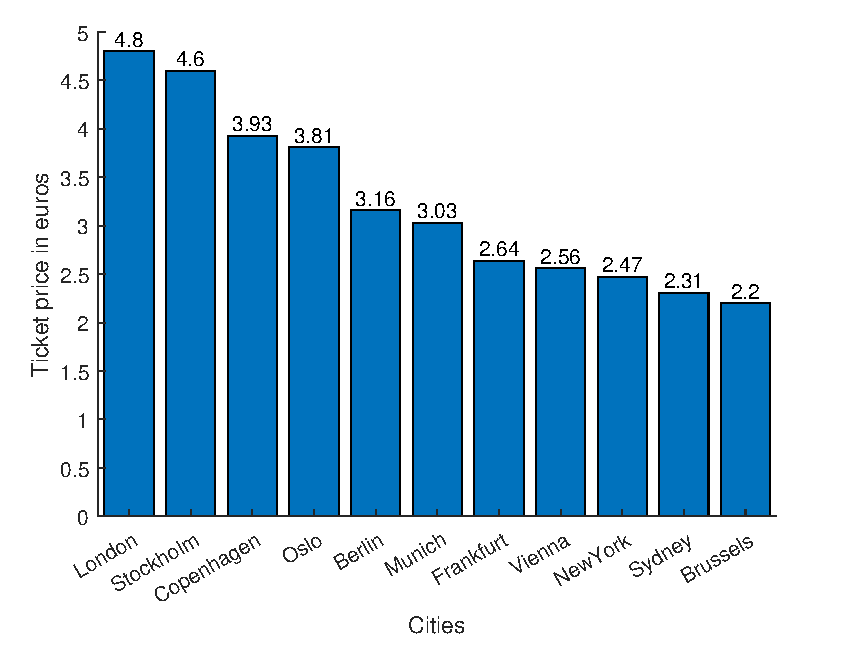
\includegraphics[height=7cm]{Images/GraphPricePT.pdf}
		\caption{Average cost for public transport (bus, tram or metro) in selected cities around the world in 2017\cite{pricesPT}.}
		\label{pricePT}
	\end{minipage}\hfill
	\begin{minipage}[c]{0.5\linewidth}
		\centering
		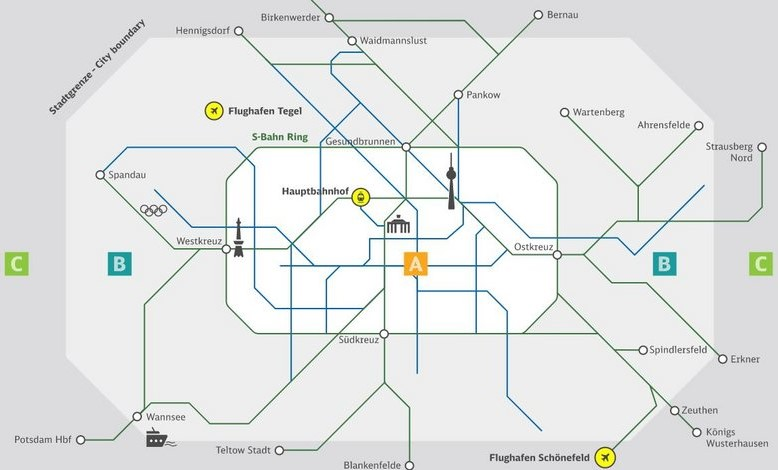
\includegraphics[height=7cm,width=0.95\linewidth]{Images/tariffZones.jpg}
		\caption{Tariff zones of Berlin demarcated according to the S-bahn train lines\cite{tarif}.}
		\label{tariffZones}
	\end{minipage}
\end{figure}
As shown on Figure \ref{tariffZones}, Berlin's divided into three tariff zones A, B and C. Zone A surrounds the city centre and the circular \textit{S-Bahn Ring}, zone B reaches the city limits and zone C includes the suburbs and Potsdam. The latter also belongs to the counties surrounding the city. Depending on the destination tickets can be bought for AB, BC or ABC\cite{tarif}. A normal one way ticket costs respectively \texteuro3.00, \texteuro3.50 or \texteuro3.80. Moreover there are short distance tickets\footnote{Short distance tickets cost \texteuro2.00 and are valid for three stops of the S- and U-Bahn or six stops of buses and trams.}, 24 hour tickets, group tickets ...  Tickets can be bought at ticket machines located at train stations, on buses, in trams, ticket counters in larger stations or the mobile app. Tickets must be validated by stamping them at the means of transport\cite{ticketing1}.

In Figure \ref{pricePT} the average cost for public transport in cities around the world is displayed. The data is based on the price of a single ticket in 2017 for public transport for a journey of approximately 10 km or at least 10 stops. The first five cities are indeed the five most expensive countries for using public transport and that includes Berlin, which makes the German capital almost 45\% more overpriced than Brussels.


\section{Bike (sharing system)}

On average, the Berliners make 44 \% of their journey on foot or by bicycle. Plus, since 2001, over 450 new crossing facilities have been constructed on the Berlin roads. and the city has currently well over 1,000 km of cycle paths, which concludes that the mobility in the city certainly is oriented towards the pedestrian and bicycle traffic. The bicycle paths can differ extensively in type: mandatory paths, off-road routes, shared bus lanes open to cyclists ... Additional \textit{Fahrradstrassen} give priority to the cyclists and make the cars slow down to 30 km/h. If a bike ticket is purchased, it's possible to take your bike on the S- and U-Bahn, on trams and on night buses\cite{MobilityCity}\cite{cycling}. \\

In the beginning of 2018 bike sharing companies were booming immensely, but now a few decent companies survived the hype. Currently there are five active bike sharing companies operating in Berlin. The best known dealers are Nextbike, Call a Bike and Lime bikes. Their prices all lay around the same number: \texteuro1-1.5 for the first 30 minutes and then \texteuro1-1.5 per 30 minutes after that. All three of them do require to drop the bike off within the S-Bahn circular ring, so it isn't possible for people who live in the suburbs to take the bike to their front door\cite{bikeshare}.


\section{Sharing systems}


	
\clearpage
\chapter{Problem and solution}
\section{Problem statement} \label{sec:problems}
\subsection{Road Congestions}
After Munich, Berlin is the city with the most traffic jams in Germany. Peak hour traffic jams are mostly caused by the commuting people. According to TomTom \cite{tomtom} data, commuting people need to add 12 minutes per 30 min. in the morning and 16 min. per 30 min. in the evening. As a normal employee works around 48 weeks per year and 5 days per week this results in an average time lost of 48 hours in the morning and 64 hours in the evening per 30 minutes additional traveling time per year. At Figure \ref{averageCongestion} the average percentages of the weekly congestion per hour are visible.

%nogal gigantische figuur, kversta datie groot genoeg moet afgebeeld worden, dus mss in appendix? of toch iets kleiner maken?
\begin{figure}[h!]
	\centering
	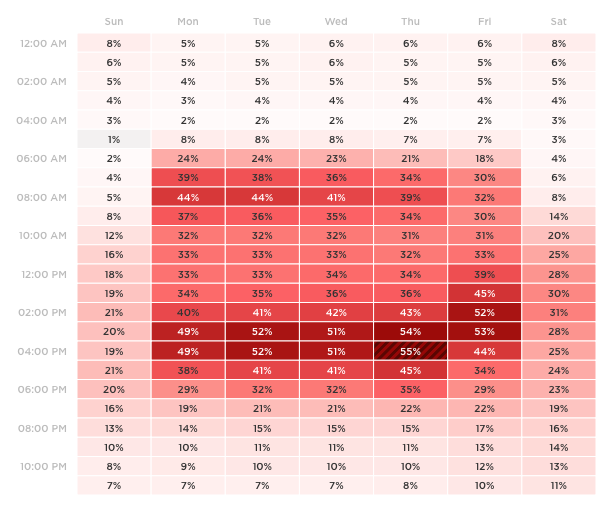
\includegraphics[width=0.55\textheight]{ProblemsFigures/TOMTOMWeeklyAverageCongestion}
	\caption{The average percentage of weekly congestion per hour in Berlin }
	\label{averageCongestion}
\end{figure}

% 'expo real': drukletters? Hoofdletter? 
\subsection{Train Delay}
A second big problem for commuting people is train delay. Typically the commuters use  the S-Bahn train (\ref{sebsec:sBahn}) to enter the city and the fast ICE train if they live at a greater distance of Berlin. As Jens-Peter Schulz, CEO of Dresdner Real Estate Investment Holding \& Chairman told in an article for expo real: 'Germany travelers cheer if their train arrives less than 10 minutes late'. Because the majority of the commuting people live near Berlin we will only analyze the S-Bahn train. People mostly complain that the complete railway system in Germany is not very flexible, once a train has a delay it just causes a lot of other delays. Especially when the train becomes very crowded, the stop time of the trains increases every time. As that train arrives in a transfer station with a delay, the other trains wait on that train so it's possible for the passengers to transfer, which results in more trains with a delay. 

\subsection{Ticket price} \label{subsec:ticketprice}
The ticket prices for public transport in Berlin are the 5th most expensive of the whole world (Figure \ref{pricePT}). As a single ticket costs around \texteuro{3.16} and the majority of the commuting people need to cover on average 14.3 Km (Figure \ref{averageComDis}) to go working. With an average fuel consumption of 4.1 L/100Km (2020) and a fuel price of  \texteuro{1,65}/L (2021), this means going to work with the car costs around \texteuro{1} --car parks payment not included. So for people that own a car and do have a car parks spot near their work, it financially seems to be more attractive to take the car. 

\begin{figure}[h!]
	\centering
	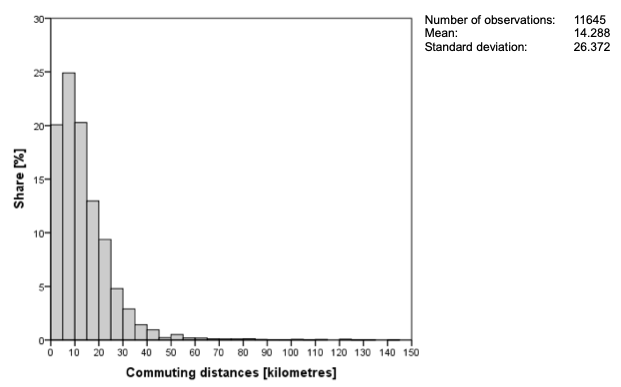
\includegraphics[width=0.55\textheight]{ProblemsFigures/averageCommutingDistance}
	\caption{The average distance the commuting people cover in 2012. }
	\label{averageComDis}
\end{figure}

\section{Proposals}
In this section some proposals are given to solve the problems discussed in section \ref{sec:problems}. There is not one right solution for these problems, but as one problem is solved this will also have an impact on the others. When trains are more reliable and cheaper, more people will use them instead of taking their car, which resolves in less road congestions. The other way around is possible as well when there are less road congestions, more people will take the car resolving in smaller delays for the trains as they will not be overcrowded. The subsections \cref{subsec:RoadTax,subsec:parkin,subsec:resSys,subsec:ticketPriceSolution} will propose an individual solutions for each problem.

\subsection{Road Pricing} \label{subsec:RoadTax}
One of the answers the the congested roads problem could be a road pricing. There are two possibilities of road pricing: either distinct prices on different roads to spread the traffic better or a dynamic road pricing that would change in function of the hours. Both can obviously be combined as well. \\ \newline
Having distinct prices on different roads is an easy way to shift traffic from one place to an other. The investment to make this possible is also relatively low. Although there's in Germany no road pricing for cars at the moment, this does not mean that it is necessary to develop a whole new system. It is possible to add just one road segment where a fee needs to be paid. Think of a tunnel, bridge or even just a road, the only investment to make is a place to stop and pay (most of the time using a barrier). Most people will automatically avoid this road and take an other one. When a congestion occurs because of an incident, the decision to make that road segment free can be made. As a result of this decision the congestion on the other road will solve much easier. The downside of this solution is when the road isn't free, it will be used much less than before and therefore the other roads will be more busy. A popular example of this solution is situated in Antwerp where the ring is very often congested. There is an other road to pass Antwerp, which has the Liefkenshoektunnel on its path. In this tunnel normally you need to pay a fee for passing. When there is a major incident on the normal ring, this tunnel is made free resulting in a smaller traffic jam.     \\ \newline
Making a variable road pricing system will spread the traffic more even through the day. Such a system means that when driving in the peak hours the price of the road is greater then when driving on more calm moments. People that do not necessary need to travel/commute at peak hours will wait or leave earlier to avoid the more expensive road pricing. It is inconvenient that a new system needs to be introduced in Germany (or at least in Brandenburg and Berlin), considering the time and work it will need to prepare, draw up and integrate. \\ \newline
These systems already exist in other countries, but are most of the time used for trucks: a receiver inside the vehicle recognizes the different pricing zones. Some examples are ViaPass in Belgium and ViaToll in Poland. The variable road pricing can be fixed (always the same every day) or dynamic (changing on the current situation). On Figure \ref{fig:dynroad} (\cite{dynRoadPrice}) it's visible that the average delay decreases a lot in the peak hours.

\begin{figure}[h!]
	\centering
	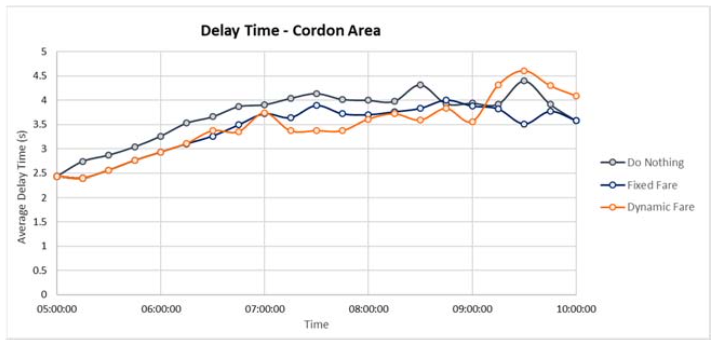
\includegraphics[width=0.55\textheight]{ProblemsFigures/dynamicRoadPricing}
	\caption{A graph that compares the average delay between different road pricing systems. }
	\label{fig:dynroad}
\end{figure}

\subsection{car parks in urban fringe} \label{subsec:parkin}
An other answer for the many traffic jams could be the so called park and ride car parks with easy accessible roads. At the moment there are a few of those in the urban fringe but you still need to pay a small amount to park there. This can only be a good solution for the road congesting problem if there is a good connection from that car park to the city centre. Some ideas are building the car parks near a U-Bahn of S-Bahn train stop, adding a bus stop at the car parks or making a bike sharing rental on the site. \\ \newline 

%de deelzinnen en zinnen staan lik allemaal los van elkaar?
The build of these car parks and additional accommodations are big investments for the city, the roads to these car parks need to be big enough to handle the peak hours. This could also mean the start of making the city centre car free as that is something happening in a lot of big cities at the moment. An example of this is the Flanders expo car parks in Ghent where you can take the tram to the city centre. 

\subsection{Variable train ticket pricing} \label{subsec:ticketPriceSolution}
A way to address the train delay problem is a dynamic train ticket price system. It would work a bit like the variable road pricing for the cars. This system would work with a magnetic card on which you put some money to pay the train ride (this can be enlarged to the whole public transport system). There would be fixed prices for each trip as it is now, except the only difference would be that the prices are divergent for different hours. This would spread the travelers more over the whole day. \\ \newline
 Now, a lot of people take the train to go to Berlin whenever they want. At the hand of this system they would first of all think when they want to take the train, so it's as cheap as possible. As we addressed in \ref{subsec:ticketprice}, the ticket price for the public system is very high comparing to other ways of commuting, therefore the prices in the peak hours shouldn't increase, but the ticket price in the non-peak hours should decrease. An additional feature to this system would be diverse subscriptions for the different times: a subscription for peak hours would be more expensive than one for non-peak hours and would be usable during non-peak hours, but not the other way around. 
 
\subsection{Train reservation system}\label{subsec:resSys}
A second solution for the train delay problem would be a train reservation system. By introducing this, the train providers can anticipate on unexpected large amounts of travelers by adding some wagons to the trains. As it's obviously not possible to make a reservation on a train mandatory, there needs to be an other way to make reservations more attractive. \\ \newline
This could be done by charging lower prices when you reserve a ticket (whether or not at least 24 hours before departure). A second way would be to guarantee a place to sit on each train, although this would be much more difficult to succeed as the rule on a train is most of the time first come first take. 

%kversta de zin niet
The system would be connected to the magnetic card, so when you pay the amount is less then it would be when you didn't reserve a spot. The system of reserving a place on a train is already used on the high speed trains as the Thalys and the TGV.  

\subsection{Political change}\label{politicalChange}
Ultimately, the politics in Germany cannot be forgotten. As it is improving at the moment, the relation politics-public transport isn't as coherent as in the other countries. The car industry in Germany is one of the biggest industries of the whole country, consequently this industry has a big influence on the German economy and politics. The car commerce is in the eyes of the politicians more beneficial to the country, resulting in a higher priority in the past and present. That's the reason why a lot of the train infrastructures are old and are being replaced at this moment. \\ \newline 
The last few years it's clear that the positive environmental impact of the public transport is very important, so much more money is invested in the public transport by the government. These new investments are on long term a good improvement against the train delays, but at short term they cause a lot of extra delays. On Figure \ref{fig:typesOfTransport} it's clear that there is still a lot of improvement possible according to more public transport and rail use compared with the car use. 

\begin{figure}[h!]
	\centering
	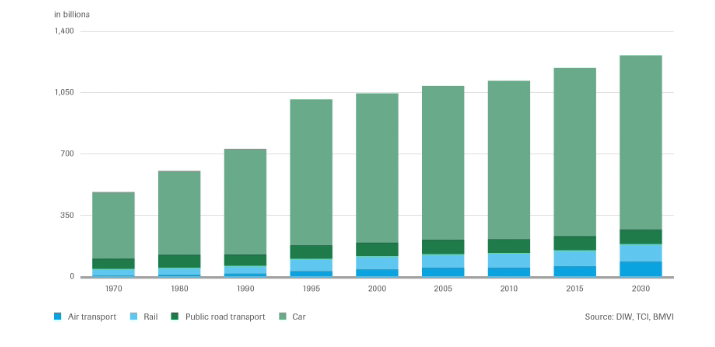
\includegraphics[width=0.55\textheight]{ProblemsFigures/typesOfTransportGermany}
	\caption{The evolution in the different used types op transport.}
	\label{fig:typesOfTransport}
	
\end{figure}



\chapter*{Conclusion}
Besluit hier typen

\clearpage

%bibliography
\nocite{dlr76743}
\bibliographystyle{plain}
\bibliography{References}

\end{document}